\documentclass[12pt,a4paper,oneside,openany]{book}


\usepackage{listings}
\usepackage{color}
\usepackage[titletoc]{appendix}

\definecolor{dkgreen}{rgb}{0,0.6,0}
\definecolor{gray}{rgb}{0.5,0.5,0.5}
\definecolor{mauve}{rgb}{0.58,0,0.82}




\usepackage{xcolor}
\usepackage{minted}
\usepackage[utf8]{inputenc}
\usepackage{tikz}
\usepackage{caption}
\usepackage{gensymb}
\usepackage{lmodern}
\usepackage{multirow}
\usepackage{booktabs}
\usepackage{array}
\usepackage{adjustbox}
\usepackage{upquote}
\usepackage{amsmath}
\usepackage{titlesec}
\usepackage[hidelinks]{hyperref}
\usepackage{fancyhdr}
\usetikzlibrary{mindmap,shadows, shapes, arrows, positioning}
\usepackage{graphicx}

%% Change these:
\newcommand{\projecttitle}{Hall of the Red Earl - An Augmented Reality Experience}
\newcommand{\projectauthor}{John Conor Kenny\\[0.2cm] Eoghan Moylan}
\newcommand{\projectadvisor}{Damien Costello}
\newcommand{\projectprogramme}{B.Sc.(Hons) in Software Development}
\newcommand{\projectdate}{\today}
%% End of things to change.



\tikzstyle{rect} = [rectangle, fill=blue!50, text width=4.5em, text centered, minimum height=4em, rounded corners]
\tikzstyle{line} = [draw, ->, very thick]
\tikzstyle{oval} = [ellipse, fill=green!50, text width=5em, text centered]

\newcolumntype{x}[1]{>{\centering\arraybackslash\hspace{0pt}}p{#1}}


\begin{document}
  \begin{titlepage}
    \begin{minipage}[t][6cm]{\textwidth}
      \centering
      \rule{\linewidth}{0.5mm} \\[0.4cm]
      { \LARGE \bfseries \projecttitle \\[0.4cm] }
      \rule{\linewidth}{0.5mm} \\[0.8cm]
    \end{minipage}
    
    \begin{minipage}[t][6.5cm]{\textwidth}
      \centering
      \textbf{\projectauthor}\\[0.5cm]
      \projectprogramme
    \end{minipage}
  
    \begin{minipage}[t][1cm]{\textwidth}
      \centering
      \textsc{\projectdate}
    \end{minipage}
      
    \begin{minipage}[t][3cm]{\textwidth}
      \centering
      \textbf{Final Year Project}\\[0.3cm]
      Advised by: \projectadvisor \\[0.1cm]
      Department of Computer Science and Applied Physics\\
      Galway-Mayo Institute of Technology (GMIT)
    \end{minipage}
  
    \begin{center}    
      
\includegraphics{img/gmit-logo.jpg}
    \end{center}
  \end{titlepage}
  \setcounter{page}{2}
  \tableofcontents
  %!TEX root = project.tex
\graphicspath{ {/Home/Users/TheShockMaster/Desktop} }

\chapter*{About this project}

\paragraph{Abstract}
The purpose of this project is to investigate the possibility of creating an Augmented Reality application for use in a local historical site. This investigation was completed by researching currently available augmented reality toolsets, selecting the most appropriate solution, and creating a prototype application using that toolset. The application will show the historical site as it once was when it was standing several hundred years ago.

By pointing a smartphone’s camera at certain predefined target points, users of the application will be able to see a 3D model of the old building generated in real time. Users will then able to walk around the the site and the augmented reality engine will be able to track the user’s location and update where they are and what they can see. The application can also provide text overlays of information about the historical site. At one location of the site, the user can get an aerial view of the old site as it once stood with a view inside the building.

By creating this application, we aim to provide a more enriching learning experience and hope to create an attraction to the site itself.
\section{Authors}
Eoghan Moylan G00298939 \\
John Conor Kenny G00301273
\chapter{Introduction}
Augmented reality is the fusion of the real world and computer based imagery. According to Milgram, an interface can be defined by the level of reality the user experiences, and, that a spectrum exists with viruality and reality being the extreme cases \cite{SPIE}.
In the middle of this spectrum lies augmented reality. Augmented reality systems are being planned in many sectors of modern industries. Liu describes augmented reality systems being used to assist in the completion of a variety of goals such as displaying instructions to workers using HMDs (Head Mounted Displays) for complex tasks such as assembly or maintenance \cite{SIGCHI}.
This project aims to create an augmented reality application for the historical site, The Hall Of The Red Earl.
The Hall Of The Red Earl is a 13th century building linked to the founding of Galway. “It was Galway’s first municipal building and was used to collect taxes, dispense justice and to host banquets” \cite{dng}. The application was designed to allow users to envision the hall as it stood during the reign of the Red Earl.
The client requested that an augmented reality app be designed and built for the hall, though no specifics in terms of platforms, technologies or methods had been specified. This resulted in a great deal of research being done on both the site and augmented reality itself. The client had, however, suggested that the app adhere to similar aesthetic to a 3D interactive map of medieval Galway that was on display in the Galway City Museum. The client had requested the app be built in order to attract more visitors to the site as the ruins are not situated on a popular street and as a result often get over looked. The clients had hoped that with the implementation of an augmented reality system tourists and archaeologists would gain an interest in the site.
Ishii describes a gap between reality and cyberspace that augmented reality systems are trying to bridge \cite{tangibleBits}. The application was designed around this principle, to bridge the divide between the 13th century ruin and the computer generated imagery of the building. Augmented reality systems allow for an experience as immersive, if not more immersive, than their virtual reality counter parts, and, as a result, augmented reality systems are often acclaimed by archaeologists who pursue a phenomenological approach to archaeology. Phenomenology is a psychology term that, when paired with archaeology, refers to the method of thought that requires the archaeologist to view the site/situation as though they were present at the time. Using augmented reality allows for a much more tangible experience for those studying archaeological sites through a phenomenological mindset.\cite{tilley} discusses the role of phenomenology in interpreting archaeology.

The objectives of the project were to research augmented realty APIs and systems that were relevant to the project, to research the Hall Of The Red Earl in order ensure that the application was historically accurate and, ultimately, to develop an augmented reality application that would allow users to envision the 13th century ruins as though they were still standing. 
\chapter{Context}
\section{Objectives}
The objectives of the project was to create an augmented reality experience for smart phones and tablets that would allow users to visualise the ruins of The Hall of The Red Earl as they were when they were intact.
The plan was to create an application that would generate an interest in the site, thus, generating an influx of visitors to the site and, therefore, a rise in donations.
The application also aims to help archaeologists studying the ruins through the school of thought known as phenomenology.

In the methodology section of this document, the programming methodologies that were used throughout the project will be covered. In this section a brief discussion will also be had in regards to the technologies used and the logic behind choosing those technologies.
In the technology review section of this document,  the various technologies that were used in throughout the development of this application will be discussed. Key components of these technologies, as well as the user interface of the application will be discussed in this section also.
In the system design section of this document the various important classes and scripts used for this application will be outlined and explained. As some of the classes in the application are not proprietary, not all will contain snippets of code.
In the system evaluation section of the document the various methods of testing will be listed and explained, as well as their effectiveness throughout the project. The performance of the project will also be measured and explained using start up times on various devices. This section will also include the various limitations and issues encountered through out the projects development.

\section{Links}
https://github.com/EoghanMoylan/AugmentedRealityApp \\
This repository contains two directories :  “Assets” and “Final Builds”. The “Assets” directory contains all of the scripts, sprites, audio and prefabs used to build the application. This directory also contains all of the Vuforia objects needed for the application to functions, these include the AR Camera module, the datasets used to define the image targets and image target prefabs themselves.
The “Final Builds” directory contains the final android build of the project. Prior to this directory, the builds were contained in a directory listed as “builds”. Going through the commits, previous versions of the application can be seen and tested. The current build is “Version 1.408.apk”. This means that this build is the  8th minor iteration of the 40th major build. Not all builds were published on GitHub, only builds tested through the various means of testing and that showcased an increase in functionality or contained significant bug fixes are listed there.\\

https://github.com/YesManKablam/2016MainDocumentation \\
This is the GitHub repository for the documentation that you are currently reading. The final output is listed as "project.pdf".\\

https://www.youtube.com/watch?v=nIjluJcAqPw\\
This is a video example of the application in action.


\chapter{Methodology}
At the very beginning of this project, we decided upon following the Agile Methodology of software development. Agile promotes adaptive planning, evolutionary development, early delivery, continuous improvement and encourages a rapid and flexible response to change. Since cutting edge technology was worked on during the course of this project, being able to change and adapt was essential. This project also involved a client. Since Agile encourages a high level of engagement with project stakeholders, the client was kept informed and shown working prototypes all the way through development.

Since this project consisted of two people working together, version control was very important. When working with cutting edge technologies, being able to backtrack and revert to a previous version is essential. For that reason, Git was selected as the source code management system. This also meant that the Git repositories could all be kept on GitHub, which is an online sharing website for Git repositories.

In order to select suitable technologies for use in this project, they needed to meet a specific set of criteria. They needed to be stable and be able to target a wide range of platforms. Since Augmented Reality frameworks are still cutting edge, any engine that is needed to to be used in order to work with the framework would either need to be easy to understand, or something that we both had experience in. For these reasons we selected the Qualcomm Vuforia framework and the Unity game engine. Qualcomm Vuforia is a stable framework that is compatible with Android, iOS and Unity. Unity is an engine that we both are quite experienced in, and it uses C\# as it’s language, which we are also quite experienced in. This decision was made during the research phase of the project. As a result it was not known what platforms the app would be deployed on. Therefore, it was in the best interest of the project that the technologies selected be cross-platform compatible. After a discussion with the client, at a later date, this decision was reinforced as, although the initial and primary build was to be Android, an iOS version of the app had not not been entirely ruled out. Android was selected as the initial and primary build due to it’s large market share and the budgetary concerns of the client. As of the time of writing, Android holds roughly a  74\% market share of all smartphone operation systems in Europe.\cite{kantra} Targeting for Android also allowed for testing on a wide arrange of devices, since any device can enable developer mode. The version of Android that was targeted was Gingerbread, Android 2.3. The reason for this is the adoption rate for Android updates are not the highest. The bellow graph from statistic.com\cite{statista} shows a breakdown of which Android versions are the most used. 

\begin{figure}[ht!]
	\centering
	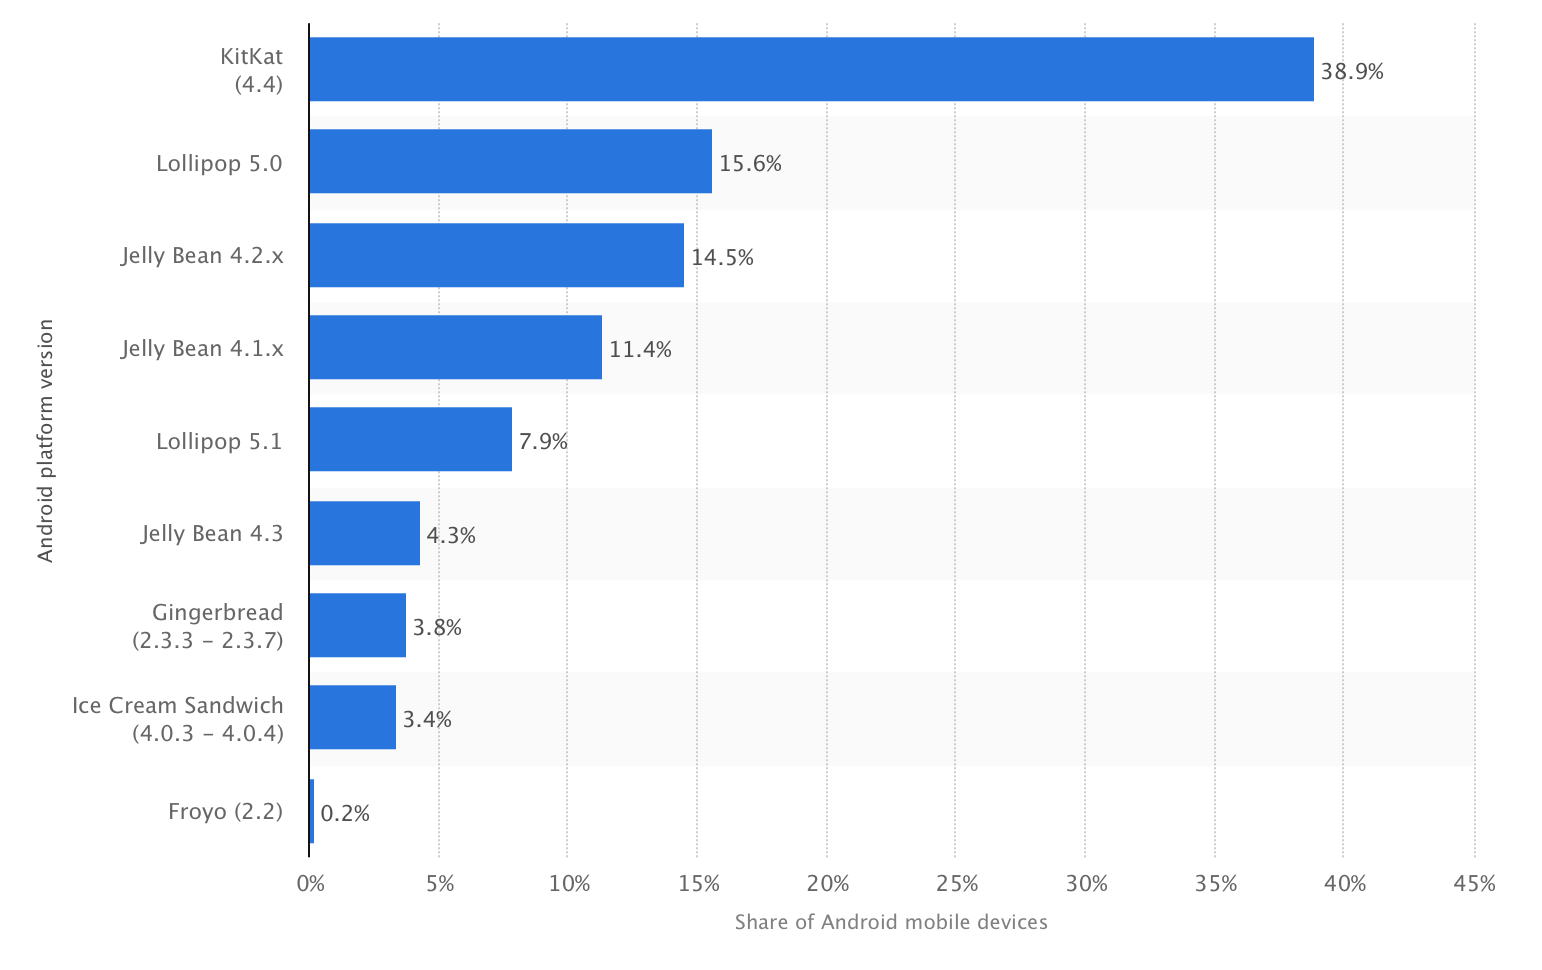
\includegraphics[width=120mm]{graph1.png}
	\caption{KitKat, Android 4.4, shows a clear lead in terms of most used Android version. \label{overflow}}
\end{figure}

As you can see, Android 4.4, KitKat, is far an away in the lead, despite it not being the latest available operation system available. The Android SDK is also completely backwards compatible. Meaning that, even though this application was built for an older version of Android, all version above 2.3 can also run that application.

\chapter{Technology Review}
\section{Vuforia}
Qualcomm Vuforia was selected as the augmented reality framework that was going to power this project. This decision was not made without extensively researching the available augmented reality engines that are available today. The other two engines which were almost selected were Metaio and AR-Media. During research, it was discovered that Metaio was purchased by Apple Inc. around May of 2015. The final date for downloading purchased licences was in December of 2015, which meant that until further notice, Metaio is no longer available for use. On the other hand, AR-Media had very little information about itself online. The documentation was not very extensive, and when developing with cutting edge technologies, documentation is needed. Vuforia’s website contains extensive documentation and a developer forum. It is for these reasons that we were pushed towards using Vuforia.

Vuforia allows for developers to create targets or markers and then position 3D models, text and much more in relation to these targets. When these targets are viewed through the camera of a smartphone or tablet, the models appear as if they are apart of the world itself. Vuforia also tracks the camera’s position in relation to the target, so if the smart phone is moved away from the target in the real world, that change is reflected in the engine.

In order to create these targets, one must first have access to a Vuforia developer account. After that is done, a License Key must be generated. The License Key is a unique identifier for each app that allows access to the Vuforia platform. The License Key is then associated with a Target Database. The database is simply a collection of the finished targets. To generate the finished targets, the Target Manager needs to be launched. According to the Vuforia Developer Library\cite{vuforiastarting}, the Target manager is compatible with a range of images and objects including: 
\begin{itemize}
	\item Image Targets are flat images, such as print media and product packaging.
	
	\item Multi-Targets are created using more than one Image Target and can be arranged into regular geometric shapes (e.g. boxes) or in any arbitrary arrangement of planar surfaces.
	
	\item Cylinder Targets are images wrapped onto objects that are approximately cylindrical in shape ( e.g. beverage bottles, coffee cups, soda cans ).
	
	\item Frame Markers provide 512 numerically encoded markers that can be used with any image. Markers may be small and you can detect and track several of them simultaneously.
	
	\item Text Recognition enables you to develop apps that recognize words from a dictionary of ~100,000 English words.
\end{itemize}

The Target Manager takes in any of these target types and then analyses them for unique identifier points. Targets are then rated on a 5 point scale for how well Vuforia will be able to recognise them.


\begin{figure}[ht!]
	\centering
	
\includegraphics[width=90mm]{raw}
	\caption{Here is a target point before it is given to the Target Manager \label{overflow}}
\end{figure}

\clearpage
\begin{figure}[ht!]
	\centering
	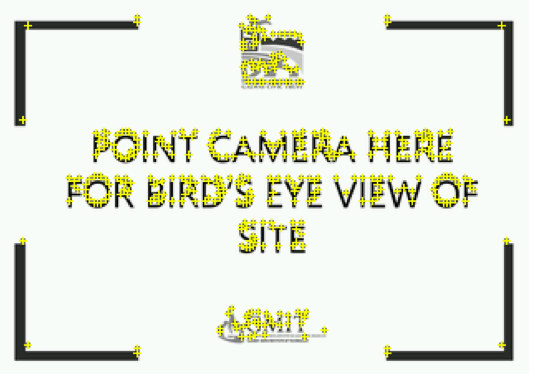
\includegraphics[width=90mm]{points}
	\caption{Here is the target point after it is given to the Target Manager \label{overflow}}
\end{figure}


Since the Target Manager recognises text and handles targets with many corners quite well, the target points that were created for this project contained both written instruction on what each point is for and a simple border. 

When all targets are finished generating, the Target Database can be downloaded and imported into another engine. The database gives you access to all of the finished image targets, which can be freely moved around within the engine. When the smartphone camera then sees one of these targets, it will move the in-engine camera to point at the recognised image target. This means that if you move the smartphone camera after seeing an image target, you are in fact moving the engine’s camera. This is how Vuforia is able to show you where the 3D models exist in relation to your position.

\begin{figure}[ht!]
	\centering
	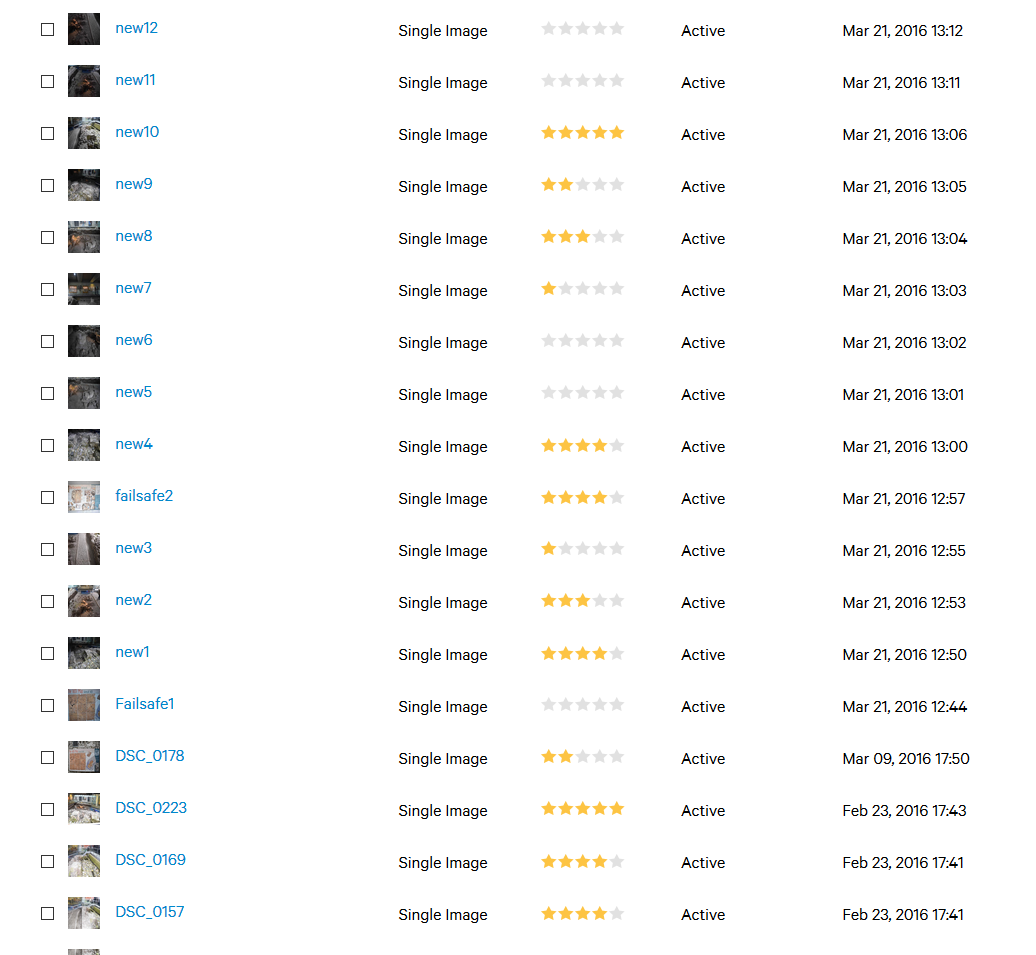
\includegraphics[width=90mm]{database}
	\caption{Here is a section of the database of target images. \label{overflow}}
\end{figure}

\clearpage

\section{Unity}
The Unity game engine was selected for this project for several reasons. It is cross-platform, well documented, active community and forum, and is compatible with Vuforia. We are both quite experienced in the Unity engine, having used in the past, which allowed us to focus on learning how Vuforia works and how to adapt it to do what we need. Unity supports three languages; C\#, UnityScript (Previously Javascript for Unity) and Boo. As of Unity 5, the option to select the Boo language has been removed from the game editor itself, but the scripts are still compatible. 

\section{C\#}
C\# is an object orientated programming language developed by Microsoft and released in the year 2000. One of the main design goals of C\# is for it to be “a simple, modern, general-purpose, object-oriented programming language.”\cite{emca}. C\# is also the go to language for Unity. In September of 2014, in a blog post on the official Unity website\cite{unityLanguage} it was shown that over 80\% of scripts created in Unity were C\# scripts. We are both quite competent at C\# too, which allowed development to focus in on the Vuforia side of the engine.

\section{Extended Tracking}
One of Vuforia’s marquee features is “Extended Tracking”. Extended Tracking allows for 3D models to remain on screen even after the original image target is lost. This means that after you point the smartphone camera away from the image target, any 3D models visible maintain their positions in respect to that target. Kincade explains that "In order for extended tracking to be possible, features that are extracted from the environment must be added to the image target feature database. The camera’s frames are then compared against the new database to determine if the camera’s relative position can be determined"\cite{kincade}
An example of this from the Vuforia Developer Library\cite{vuforiaExtended} shows originally the target marker and the 3D objects which are tied to said marker.

\begin{figure}[ht!]
	\centering
	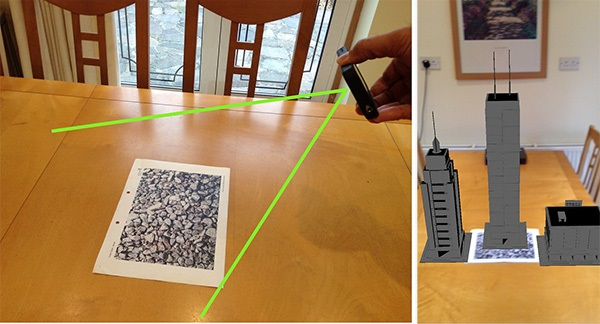
\includegraphics[width=90mm]{extended1}
	\caption{On the left is a target and a smartphone camera’s vision cone. On the right is what can be seen on the smartphone’s display.
		 \label{overflow}}
\end{figure}

\clearpage

\begin{figure}[ht!]
	\centering
	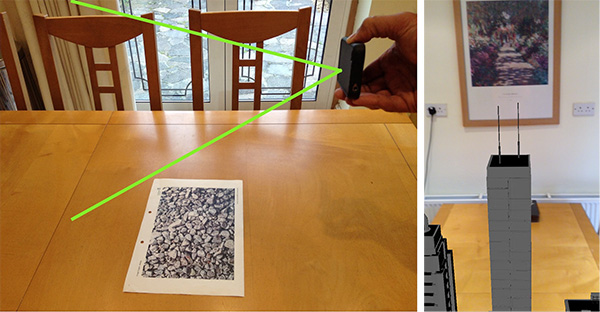
\includegraphics[width=90mm]{extended2}
	\caption{On the left you can see the smartphone is now unable to see the image target.
		On the right you can see that the 3D models have not disappeared, but rather Vuforia has extrapolated the new position of the 3D model based on where the image target was last seen.
		 \label{overflow}}
\end{figure}


The Extended Tracking feature was exactly what was needed in order to map the 3D model of the old site to the new location. The site was extensively photographed and the resulting images were then ran though the Target Manager. The best targets where then used to map out the site in the Unity engine, where the 3D model was then placed in relation to those targets. The smartphone camera was able to recognise these natural targets, and it would then display the 3D model of the old site. When a natural target was then lost, extended tracking helped bridge the gap between the previous target and the next natural target the user would see.


\section{User Interface}
Van Dam describes interfaces as an “intermediary between the users intent and the execution of that intent”  and with that principle in mind they should be treated as a necessity and not a feature\cite{avd}. Augmented reality systems often require alternative user interface designs to standard desktop GUIs (Graphic User Interfaces), known as W.I.M.Ps (Windows, Icons, Menus, Pointers), as they can “constrain the user due to limited screen space and interaction bandwidth”\cite{spacetop}. This project was designed with the intention of keeping the UI (user Interface) as unobtrusive and immersive as possible. As a result all of the assets used in the UI were created specifically for this project. The UI in this project consists of a number of buttons which are placed along the top of the screen. The designs were based on the UI used by other popular apps and were purposefully kept minimalistic in order to avoid confusion as to there purpose, as well as in order to keep the user immersed in the augmented reality of the app.
Bai claims that the use of mobile devices in collaboration with augmented reality systems results in issues with stability, as the user struggles to hold the device wit hone hand and interact with the interface with the other\cite{interactiveMethods}. Lee mirrors this concern and states that frequent shaking of the device results in erroneous operations\cite{freezesetgo}.

\begin{figure}[ht!]
	\centering
	
\includegraphics[width=90mm]{mainMenu}
	\caption{Here is the Main Menu of the Application. \label{overflow}}
\end{figure}

With these concerns in mind, the UI for this project was designed to require minimal input from the user. This resulted in decreased shaking and occlusion of the screen, though it did not entirely abolish it.
At first the UI was designed with the intention of it being semi transparent. However, this idea was quickly abandoned as it was found that the interfaces blended into the background to a degree which made it difficult to understand the interactions the user would be required to make.
Another section of the UI are the facts about the site which appear over the various sections of the ruins. These were included to explain to the user the history of the site without the need for a guide. The designs of these facts were kept minimal and follow the same colour scheme as the rest of the UI. They can also be toggled on and off as some users may find them unimmersive.

\begin{figure}[ht!]
	\centering
	
\includegraphics[width=90mm]{mainMenu}
	\caption{Here is the UI running in the Application. \label{overflow}}
\end{figure}

\chapter{System Design}
\begin{figure}[ht!]
	\centering
	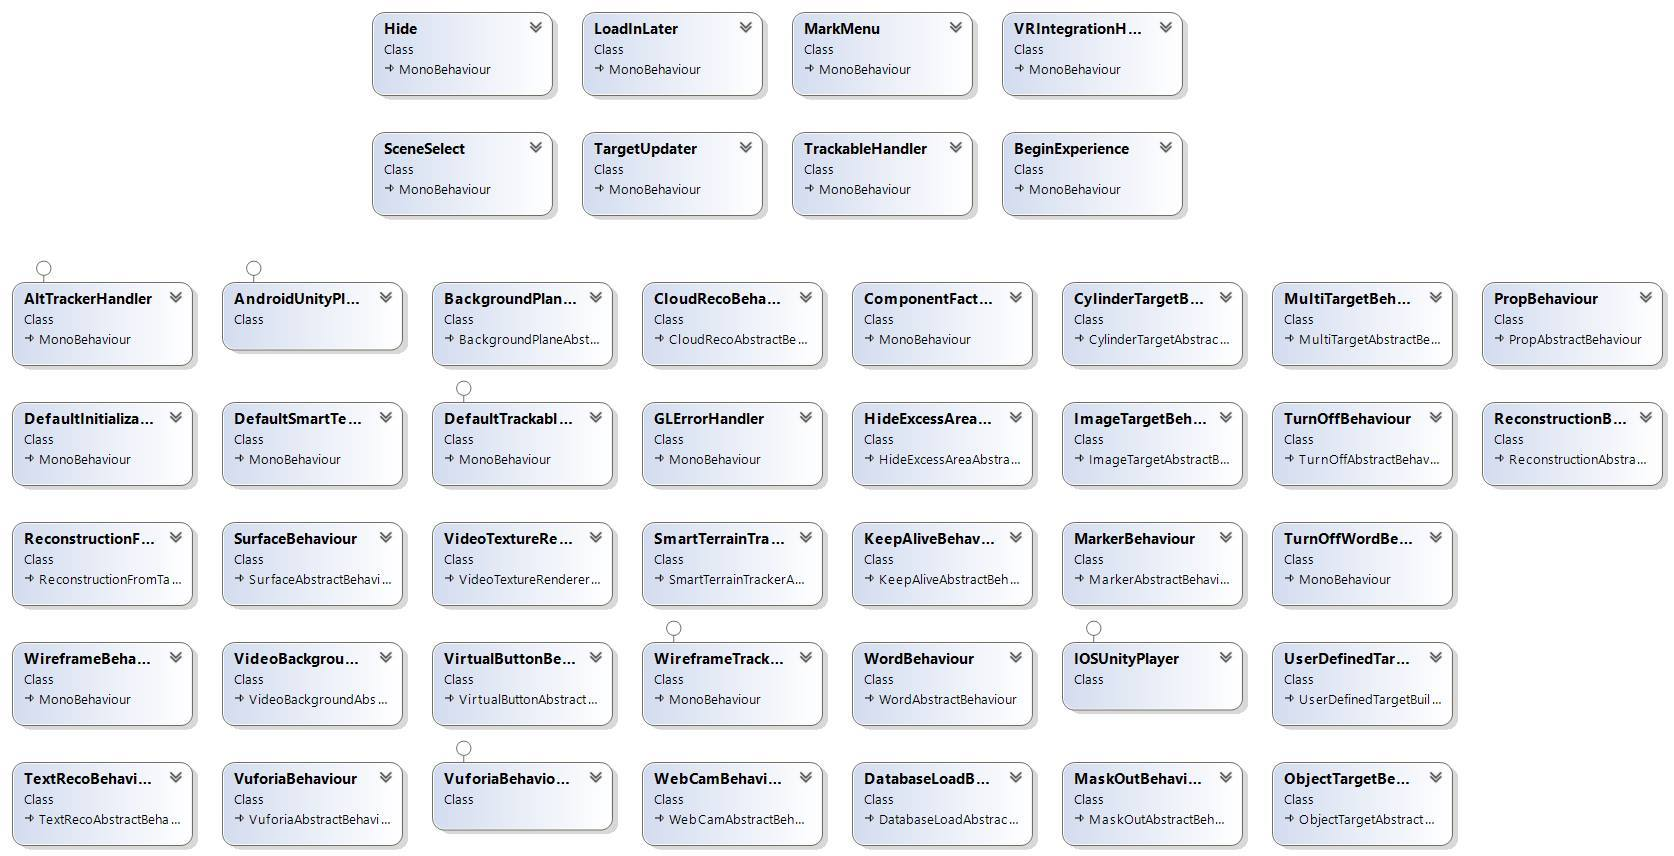
\includegraphics[width=150mm]{uml.jpg}
	\caption{A simple caption \label{overflow}}
\end{figure}

\section{HIDE}
There is an instance of the Hide class in the AltTrackerHandler. The method invisible or the method visible are called in the OnTrackingFound()/OnTrackingLost() methods. This Hide class instance is attached to a gameobject with the tag “Building”. This gameobject has several child objects attached to it with an identical tag. Originally the Hide class would then deactivate the renderer of all of the gameobjects with tag “Building”.  However, this proved to cause issues with various versions of Unity and Vufoira. Instead the script was altered to deactivate the parent object, and, as a result, all of it's child objects. This script was developed to prevent models being loaded in when no image target was detected and to load models out of memory when the AltTrackerHandler called the OnTrackingLost() method.

\section{BEGIN EXPERIENCE}
The BeginExperience script is attached to the camera in the Unity scene. The camera's culling mask is set to not include object with the tag “hall”. This ensures that the model does not appear before the image target is detected. The script accesses the global variable “begun” once per frame. If the variable is set to 1, then the BeginExperience script will add the model of the Hall to the culling mask. This ensures that the camera will show the model. This variable is set to 1 in the DefaultTrackerHandler method OnTrackingFound(). The BeginExperience script also allows for gameobjects to be activated when a target is detected. This was initially used to load in the UI after the image target was detected but was later removed due to poor user experience. 

\begin{lstlisting}
private void setUpBegining(){
   cam.cullingMask |= 1 << LayerMask.NameToLayer("Hall");
   toLoad.SetActive(true);
}
\end{lstlisting}

\section{ALT TRACKERAHNDLER/DEFAULTTRACKERHANDLER}
Both of these scripts are very similar and are based off of the initial DefaultTrackerHandler class supplied by Vuforia. The classes are handlers that implement the ITrackableEventHandler interface. The classes have an instance of the TrackableBehaviour class that determines whether a trackable event has occured. The Start() methods of these classes are called when the class is first triggered. In this method the trackable event is registered if it has occured. The two key methods in these classes are the OnTrackingFound() method and the onTrackingLost() method. These methods are called when when trackable event is detected, e.g an image target is in view of the camera, an trackable object is in view of the camera etc. The AltTrackerHandler is used to trigger the Hide script while the DefaultTrackerHandler will set the “begun” variable. Both of these scripts will also enable/disable the colliders and renderers of the children attached to the script. In this project that feature is not implemented.

\begin{lstlisting}
void Start(){
   mTrackableBehaviour = GetComponent<TrackableBehaviour>();
   if(mTrackableBehaviour){
      mTrackableBehaviour.RegisterTrackableEventHandler(this);
   }
}

private void OnTrackingFound(){
   if(hide != null){
      hide.GetComponent<Hide>().visible();
   }
   ...
}
\end{lstlisting}

\section{VIDEOTEXTURERENDERER \& VideoBackgroundBehaviour \& BackgroundPlaneBehaviour}
BackgroundPlaneBehaviour class creates a mesh plane which is attached to the camera. The plane is then painted with a texture created by the VideoTextureRenderer. The VideoTextureRenderer creates a texture comprised of the feed taken from the devices camera. The VideoBackgroundBehviour handles the native video background rendering and needs to be attached to a camera object.
In the space between the background video plane and the camera is where our models are placed. This creates the illusion of the models appearing as a part of the camera's image, making them seem part of real life.

\section{KeepAlive \& DataBaseLoadBehaviour \& VuforiaBehaviour}
The VuforiaBehaviour script determine the platform the application is running on and creates a singleton “getter” to the VuriaBehaviour object. It then adds the ComponentFactory which creates all of the necessary objects needed for Vuforia to function.   
The KeepAlive behaviour allows for Vuforia objects to be loaded across various scenes. This reduces the amount of loading needed when switching between scenes. It also makes it possible to share datasets and targets (of different types) across multiple scenes. However, in order to function it must be attached to gameobject that also has the VuforiaBehaviour script attached to it. The DatabaseLoadBehaviour determines what datasets are to be loaded in the scene and whether or not they are to be activated. The script allows for multiple datasets to be loaded and activated at a time. By default the datasets (which are stored in XML and DAT files) are located in the StreamingAssets folder.

\begin{lstlisting}
protected void Awake(){
   IUnityPlayer unityPlayer = new NullUnityPlayer();
   
   // instantiate the correct UnityPlayer for the current platform
   if (Application.platform == RuntimePlatform.Android){
      unityPlayer = new AndroidUnityPlayer();
   }
   else if (Application.platform == RuntimePlatform.IPhonePlayer){
      ...
   }
   
   gameObject.AddComponent<ComponentFactoryStarterBehaviour>();
}
   
public static VuforiaBehaviour Instance{
   get
   {
      if (mVuforiaBehaviour == null){
         mVuforiaBehaviour = FindObjectOfType<VuforiaBehaviour>();
      }
      return mVuforiaBehaviour;
   }
}
\end{lstlisting}

\chapter{System Evaluation}
\section{Testing}
In order to ensure that the application performed as intended, testing was done at regular intervals for the various components. These intervals varied depending on the component.
Testing was broken down into three main categories: Image targets, natural image targets and finally user experience.
Image target tests were the simplest of the tests to conduct. This resulted in short intervals between tests, usually two or three days. These forms of tests were also conducted after each build of the application. These tests involved using the designed image targets as the targets for the application. As there were a total of only four designs, these forms of tests were often used just to verify that the application was working as intended. To conduct these tests the designs were placed on a flat surface and the smartphone's camera pointed towards them. In general, the results would indicate if the model was scaled properly, was in the correct position and that the application had been built properly.

The natural image target tests were the most complicated and difficult to conduct. This is as a result of a number of factors. A notable issue is that this form of testing could only be conducted at the site itself, as the image targets were directly linked to the ruins. Initially, attempts were made to conduct these tests using a similar technique as the image target tests, and, though these yielded moderate results, it was concluded that this alternative method was ultimately ineffective and not wholly representative of the site. These forms of testing often resulted in the most valuable information. The results highlighted issues with scale and positioning also, but more importantly showcased the issues with lighting, design of the application and the, eventually, the positions that designed image targets needed to be placed.

The final category of testing was user experience testing. These tests were simple to conduct, though their results were often difficult to interpret. These tests were conducted by giving the application to friends and family as well as image targets. The users were not told how to use the application as it was believed that this would resulted in a fairer result. These results varied as some users understood the application immediately and had little criticism, while others had difficulty understanding the application's layout and design. These results were taken into consideration as the project continued forward and the designs were altered accordingly. These forms of tests resulted in vital information in regards how the application was used. A reoccurring issue that these tests highlighted was the need for a starting point as most users would not point the camera at the same spot when entering the site. This culminated in the need for designed image targets. 

\section{Performance}
Performance of the application varied to a degree depending on the phone or tablet the application was installed on. This was somewhat intentional as the application was designed to deployed on a wide range of android devices, and it was understood that older models would be slower. However, overall the application performs relatively well on older devices and very well on newer devices.
Initially the same virtual “AR Camera” was used in multiple scenes in the Unity engine. Vuforia allows for this via a script called “Keep Alive Behaviour”. This script keeps the image target datasets and other objects loaded in memory. This resulted in a long loading screen at start-up, but a very quick transition between the various scenes. This approach was quickly abandoned after it became apparent that there was no intuitive means of placing the “AR Camera” within the scenes on loading in. It also resulted in a number of issues where scenes were not running properly, in some cases crashing, as the camera would not spawn in as well as resulting in models not loading in the correct position.
It was then decided that a new camera instance be created in each scene which only loaded in datasets that were required in that scene. This resulted in slower transition times between scenes, but an overall more stable application.
In order to reduce the memory required by the application all of the image targets were shot at a high resolution but converted to much lower quality image through Photoshop. Though the difference in image quality was not particularly noticeable to the average viewer, the size of these images were reduced from an average of 28-30 MB to 300-500 KB. 
Performance testing was also carried out on the final build. Using a range of different Android devices, the time it took to load the application from the homescreen was recorded. The left column indicates the model of phone, while the right column is the result time in seconds.

\begin{center}
	\begin{tabular}{ |c|c|c| } 
		\hline
		HTC M8 & 04:73 \\ 
		Motorola Moto G (2nd gen) & 06:39 \\
		Motorola Moto G (1st gen) & 4:70 \\ 
		Samsung Galaxy S7 Edge & 02:67 \\ 
		Samsung Galaxy Tab S2   & 03:96 \\ 
		Sony Xperia Z2 & 02:80 \\ 
		\hline
	\end{tabular}
\end{center}

\section{Issues and limitations}
Throughout the development of the application a number of issues with both the technologies used and the design approach became apparent. Though these varied in severity, they were addressed and removed or at the very least reduced in scale and intensity.
At a late stage in the project it became apparent that relying solely on natural image targets to track the ruins was completely infeasible. This is a result of a number of factors.
Firstly, as the ruins are an outdoor location, lighting became an increasing issue as the project progressed. The light enters through the windows on one side of the site and through an open area on the other. This results in the critical natural image targets, namely the walls of the ruins, being subject to changing light. These changes in light cause changes in the shadows cast by the site and, therefore, altering them to the shadows in the image targets set up in Unity. Although the colours of the image targets are not taken into account by the Vuforia engine, these changes in shadow alter the image captured by the camera, resulting in the application not registering them as valid image targets.
Secondly, as Vuforia uses the detected corners on images as tracking points, certain areas of the ruins were unusable as targets. The empty space and pillars that mark the interior of the Hall were the least effective as image targets. Vuforia rarely registered these spaces as image targets, making them very unstable and completely unreliable. For these reasons it was decided that a number of image targets would have to be designed as a fail-safe in the even that the ruins become unusable as targets.
As discussed earlier these image targets later became the starting points of the application in order to avoid confusion.

\begin{figure}[ht!]
	\centering
	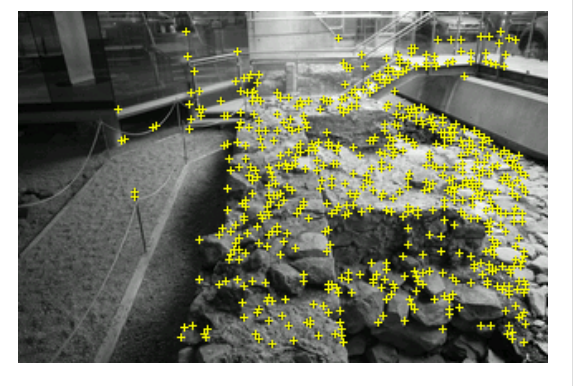
\includegraphics[width=90mm]{goodTarget}
	\caption{Here you can see a natural target that works very well.
		\label{overflow}}
\end{figure}


\begin{figure}[ht!]
	\centering
	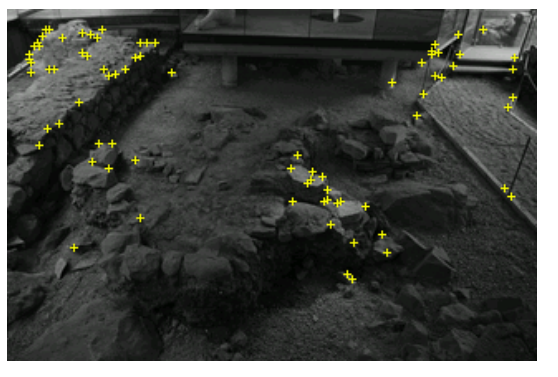
\includegraphics[width=90mm]{badTarget}
	\caption{Here you can see a poor natural target.
		\label{overflow}}
\end{figure}
The placement of the image targets was in itself an issue that arose in the final days of the project. While recording a video of the final prototype application, it became very apparent that the correct placement of these targets would deciding factor as to whether the application would function as intended or not. As Vuforia sets the world centre of the Unity scene as the first target detected, it was crucial that the starting point image targets be placed in the correct positions. On the day of recording the video wind and rain had been present. As the targets being used were temporary they were not on flat surfaces and were not protected from the rain. This meant that placing of the targets had to be done as quickly as possible. Though a rough estimation had been done in the Unity engine as to areas of the ruins that targets would be placed, it was very difficult to match these areas in the actual ruins. This resulted in many trial and error attempts to get the model lined up perfectly. Upon the release of the final version, it will be critical to success of the application that these targets are placed in the correct position.

\begin{figure}[ht!]
	\centering
	\includegraphics[width=90mm]{sitemap}
	\caption{Here is the map of the site with suggested locations for the placement of the image targets.
		\label{overflow}}
\end{figure}

The Vuforia engine itself has created quite a few problem through the project. Although most had been dealt with, one reoccurring issue that had to be worked around was Vuforia not updating the current target. Though this was a rare occurrence, Vuforia has an ongoing issue whereby it does not update the current image target, resulting the previous target being registered as the current target. This causes the model to load in incorrectly. A number of steps to combat this were taken such as clearing Vuforia's image cache each time a new target was discovered. However, these steps resulted in more issues further and, eventually, the only work around available was to add a refresh button which would reload the scene should the issue occur.

Version control and code sharing also turned out to be quite a huge challenge during this project. Unity can at times have issues when used with Git, especially if an incorrect “.gitignore” file is used. Vuforia also presented some issues with Git compatibility. When combined, Unity would crash whenever the Vuforia camera was opened and inspected after it had been passed through Git. In order to get around this, codebases were kept separate from each other until they were needed to be combined at the very end of development. A benefit of using the Unity game engine is that any scripts or game objects created are easily exportable to be used in another project. This means that while the codebases were kept apart, assets and code can be freely swapped between said codebases relatively easily without too much difficulty.

\chapter{Conclusion}
The intention of this project was to create an augmented reality application for the Hall Of The Red Earl which would allow users to envision the ruins as they were in the 13th century. The aim was to generate an interest in the otherwise unknown ruins. Thus, attracting new visitors to the site in the form of tourists as well as archaeologists. Using an augmented reality system, the attraction of archaeologists interested in phenomenology was also seen as an important by-product of the application.

The development of the application was achieved by using various cutting edge and established technologies such as Vuforia and Unity which were well researched an adapted to the needs of the project.
These technologies allowed for the possibility of the development of a cross platform application, resulting in more users and, therefore, visitors. Unfortunately, due to budgetary constraints, and android build was the only version of the application available on the completion of the project. However, due to the means through which the application was developed, the possibility of an iOS build in the future is entirely plausible.

The application developed uses a unique method for tracking the ruins. The application uses both the ruins and designed image targets to track and render models accordingly. This fusion tracking allows for a more stable experience and has to duel effect of providing functionality to the application in low light and in poor weather conditions. This is crucial for this site in particular as the ruins are partially outdoors.

Issues with the Vuforia and Unity engines themselves persist in the final build of the application, as they are both proprietary and therefore unchangeable. However, these issues are reduced in severity with a number of additions to the application. Issues with the image targets were resolved by redesigning the image targets in question. In order to overcome issue with GitHub the two sections of the project were placed on separate repositories and combined at an appropriate time. This resulted in compatibility issues which had to be overcome. These issues were a result of different versions Unity and Vuforia being used, but were overcome by the alteration of certain classes.

The UI was designed specifically for the application and each icon was drawn in Photoshop to ensure a uniform and professional aesthetic throughout the application. In order to ensure that the UI was as easy to understand and as intuitive as possible, much testing was done on it before it was published to GitHub. This ensure that the majority of users understood the layout and the functionality of the buttons.

Through regular commits to the GitHub and iterations of the application, the agile methodology was implemented whenever possible. This can also be seen in the iterative testing and regular meetings with both the client and the project team. Testing the application was a difficult task as the application was designed to only work in one location properly. This was overcome through various testing methods that tested various aspects of the application without the need to be present at the site. This means most of the application was subject to regular testing and aspects that had less frequent testing did not require the same level of attention.

In conclusion, though there were difficulties and issues that the project and team were subject to throughout development, the final application meets the clients requirements, uses cutting edge technologies and generates an immersive, stable and interesting augmented reality experience.

\begin{appendices}
\chapter{Links}
https://github.com/EoghanMoylan/AugmentedRealityApp \\
Source code.\\

https://github.com/YesManKablam/2016MainDocumentation \\
Documentation source.\\

https://www.youtube.com/watch?v=nIjluJcAqPw\\
Video demonstartion.\\
\end{appendices}
  \bibliographystyle{ieeetr}
  \bibliography{mybib}
\end{document}
